%
%

%%-----------------------------------------------------
%%-----------------------------------------------------
\section{Mapas, mapas, mapas}

%%-----------------------------------------------------
\begin{frame}
\frametitle{OpenStreetMap}

\begin{center}
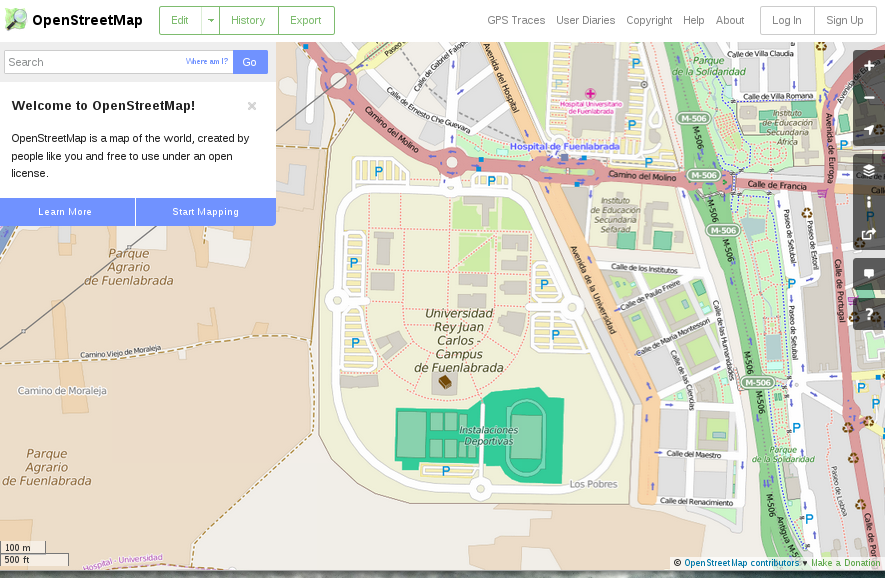
\includegraphics[height=7cm]{figs/openstreetmap}
\end{center}

\begin{flushright}
  \url{http://www.openstreetmap.org/}
\end{flushright}
\end{frame}

%%-----------------------------------------------------
\begin{frame}
\frametitle{OpenStreetMap (editando con iD)}

\begin{center}
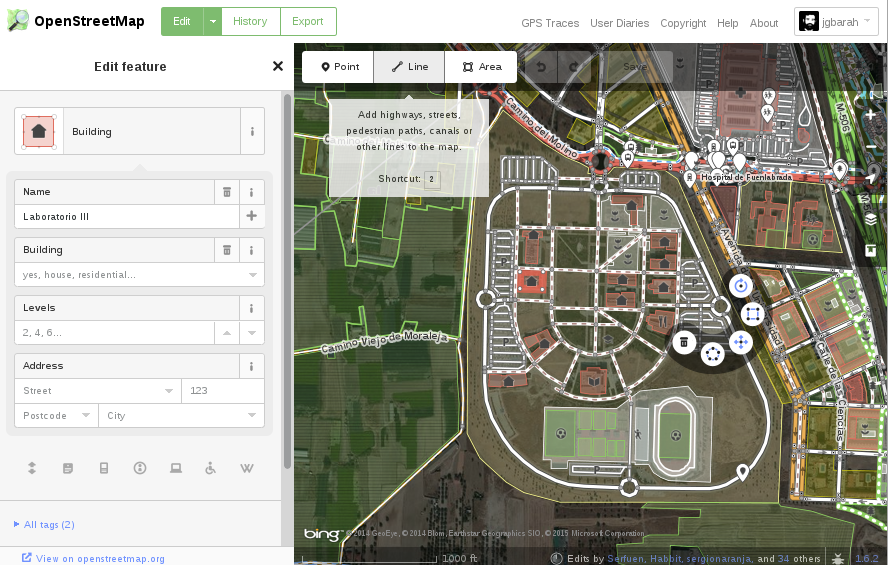
\includegraphics[height=7cm]{figs/openstreetmap-id}
\end{center}

\end{frame}


%%-----------------------------------------------------
\begin{frame}
\frametitle{Algunas curiosidades...}

\begin{itemize}
\item Servicios basados en OpenStreetMap \\
  \begin{footnotesize}
  \url{http://wiki.openstreetmap.org/wiki/List_of_OSM-based_services} 
  \end{footnotesize}
\item Software que usa OpenStreetMap \\
  \begin{footnotesize}
  \url{http://wiki.openstreetmap.org/wiki/Software\#Mobile_Devices} 
  \end{footnotesize}
\item Ejemplo de app Android: NavFree \\
  (permite off-line maps) 
\item Cómo editar OpenStreetMap \\
  \begin{footnotesize}
  \url{https://www.youtube.com/watch?v=N_00vAPjSkw} 
  \end{footnotesize}
\item 10 años de OpenStreetMap (video) \\
  \begin{footnotesize}
  \url{https://www.youtube.com/watch?v=7sC83j6vzjo} 
  \end{footnotesize}
\end{itemize}

\end{frame}

